\section{Implementation der Dekompression}
Der JHelioviewer lädt eine Folge von komprimierten Simulationen über eine Internetverbindung und muss diese vor der Visualisierung dekomprimieren. Das Herunterladen und die Dekomprimierung sind zeitaufwändige Operationen und führen zu Wartezeiten beim Benutzer. Um die Operationen zu beschleunigen werden im Ist-Zustand die Simulationen im Voraus asynchron heruntergeladen. Somit sind die Daten bereits im Arbeitsspeicher, bevor die Daten dekomprimiert und visualisiert werden.\\
Die Dekompression wird direkt vor der Visualisierung durchgeführt. Bei einer Animation der Feldliniendaten führt das zu einer bemerkbaren Verzögerung bei jedem Wechsel. Um die Qualität der Animation zu verbessern und die Wartezeit weiter zu verkürzen wurden folgende Massnahmen umgesetzt:
\begin{enumerate}
	\item Asynchrone Dekompression.
	\item Vorladen der Dekomprimierten Feldlinien.
	\item Caching von Komprimierten und Dekomprimierten Feldlinien.
\end{enumerate}

\subsection{Software Architektur}
\begin{figure}[!htbp]
	\center
	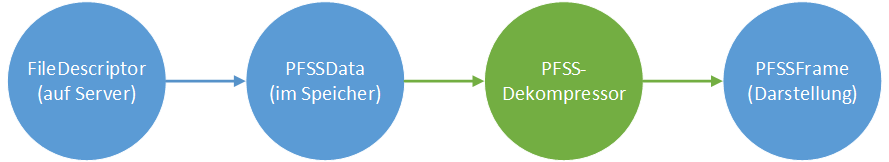
\includegraphics[width=0.6\textwidth,height=6cm,keepaspectratio]{./pictures/implementation/dataflow.png}
	\caption{Zustandsdiagramm der Feldliniendaten}
	\label{implementation:architektur:datenfluss}
\end{figure}
Die Daten der Feldlinien durchlaufen im JHelioviewer vier Zustände, welche durch vier Klassen abgebildet wurden. Die Klassen sowie die Zustandswechsel sind im Diagramm der Abbildung \ref{implementation:architektur:datenfluss} dargestellt. Die Klasse FileDescriptor repräsentiert eine Simulation von Feldlinien auf dem Server. In diesem Zustand sind die Daten bereit für das Herunterladen. Die folgende Klasse PfssData symbolisiert Feldlinien, welche in den lokalen Arbeitsspeicher geladen wurden. In diesem Zustand sind die Daten noch komprimiert und nicht bereit für eine Visualisierung. Die Klasse PfssDekompressor ist ein Zwischenzustand und stellt den Wechsel von komprimierten zu unkomprimierten Daten dar. Da der Zustandswechsel aufwändig ist, wird es durch eine eigene Klasse abgebildet. Die letzte Klasse PfssFrame repräsentiert die dekomprimierten Feldlinien. In diesem Zustand sind die Daten bereit für die Darstellung. Die Darstellung wird ebenfalls von der PfssFrame Klasse übernommen.

\subsubsection{Vorladen und Caching von Komprimierten und Dekomprimierten Feldlinien}
Um die Animation der Feldlinien möglichst Unterbrechungsfrei zu gestalten, werden die komprimierten und dekomprimierten Feldliniendaten vorgeladen und zwischenspeichern. Mit dem Vorladen wird erreicht, dass der Wechsel von der Visualisierung einer Simulation zur Nächsten möglichst ohne Unterbrechung durchgeführt werden kann. Das Caching hilft, wenn der Benutzer einen gespeicherten Zeitpunkt der Animation nochmals darstellen möchte. Die Implementation ist im Diagramm der Abbildung \ref{implementation:architektur:caching} dargestellt.

\begin{figure}[!htbp]
	\center
	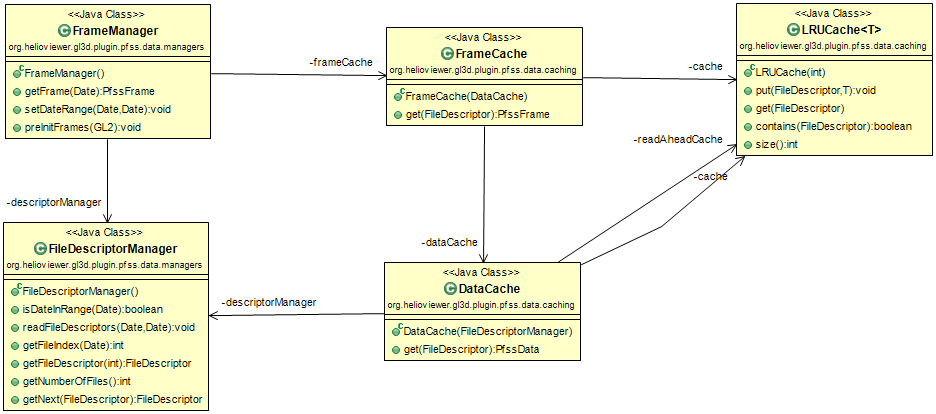
\includegraphics[width=1\textwidth,keepaspectratio]{./pictures/implementation/architectureCache.png}
	\caption{Diagramm der Implementation vom Vorladen und Caching}
	\label{implementation:architektur:caching}
\end{figure}
Die Klasse FrameManager ist zuständig für das Vorladen der dekomprimierten Daten, der PFSSFrame Objekte. Das Caching wird in der FrameCache Klasse umgesetzt. Die Klasse DataCache ist für das Vorladen und Caching der komprimierten Daten zuständig. Die FileDescriptor Objekte repräsentieren eine Feldliniensimulation auf dem Server, der FileDescriptorManager ist zuständig für das Auffinden der Simulationen.\\
Die Klasse FrameManager repräsentiert die Facade der Vorladens- und Caching- Implementation. Sie abstrahiert das Zusammenspiel der verschiedenen Caches und den verschiedenen Zustände der Feldliniendaten und bietet eine vereinfachte Schnittstelle an.\\
Die Vorladen und Caching Implementation der PfssFrame Objekte wurde in zwei Klassen aufgeteilt: Die PfssFrame Objekte müssen vor der Visualisierung Ressourcen der Grafikkarte allozieren. Nachdem ein Objekt visualisiert wurde, müssen die Resourcen freigegeben werden. Der FrameManager ist zuständig die Allozierung anzustossen und die Freigabe sicherzustellen.\\
Die PFSSData Objekte können vom Garbage-Collector verwaltet werden. Das Vorladen kann mit einer weiteren Instanz des LRU-Caches umgesetzt werden und wurde direkt in der DataCache Klasse implementiert.

In dieser Arbeit wurde ein Least-Recently-Used (LRU) Cache Algorithmus verwendet. Der LRU-Cache löscht das am längsten nicht verwendete Objekt, wenn der Cache gefüllt ist. Da der JHelioviewer im allgemeinen Fall sequenziell Objekte verlangt, kann der LRU Cache mit einer First-in-First-Out Queue implementiert werden. Das Objekt, welches am längsten nicht  verwendet wurde, ist das Letzte in der Queue. Ein LRU-Cache funktioniert in diesem Anwendungsfall optimal, wenn die Anzahl Objekte grösser ist, als der Cache. In einem Spezialfall ist der LRU-Algorithmus nicht optimal. Wenn der JHelioviewer zur letzten Simulation der Feldlinien angekommen ist, wird an wrap-around durchgeführt und wieder die erste Simulation verlangt. Wenn der Cache $n-1$ von $n$ Simulation abspeichern kann, so löscht der LRU-Algorithmus immer die Simulation, welches als übernächstes abgefragt wird. Das führt dazu, dass gleich viele Cache-Misses geschehen, als wenn der Cache wesentlich kleiner währe.

\subsubsection{Asynchrone Aufrufe mittels Executor Services}
Im Diagramm der Abbildung \ref{implementation:architektur:caching} zu sehen ist, wird das Erstellen von PFSSData und PFSSFrame Objekten jeweils von zwei Klassen übernommen werden, den Creators. Sie sind zuständig für das asynchrone Herunterladen und Dekomprimieren der Feldliniendaten. Die asynchrone Ausführung ist mit dem Java Executor Service umgesetzt. Der Executor Service verwaltet und begrenzt die Anzahl an Threads welche die Aufrufe bearbeiten, sodass auch bei hoher Auslastung ein möglichst hoher Durchsatz erreicht wird. Im Ist-Zustand wurden alle asynchronen Aufrufe jeweils in einem eigenen Thread ausgeführt. Bei hoher Auslastung steigt der Verwaltungsaufwand der Threads und bremst das System.\\
Für die asynchrone Ausführung, müssen die Klassen aus Abbildung \ref{implementation:architektur:datenfluss} Threadsafe implementiert sein. Die FileDescriptor Klasse kann als Immutable einfach Threadsafe umgesetzt werden. Für die Klassen PfssData und PfssFrame wird der Ablauf komplexer: Ein PfssData Objekt existiert, sobald das Herunterladen der Daten asynchron gestartet wurde. Die Daten können bei der Verwendung des Objekts komplett, teilweise oder gar nicht heruntergeladen sein. Dasselbe Problem gilt für die PfssFrame Objekte. Hier wird eine Wait-Signal-Logik umgesetzt. Sobald Ressourcen verlangt werden, wie die komprimierten Feldliniendaten des PfssData Objektes, wird ein non-busy waiting durchgeführt. Der aufrufende Thread wird schlafen gelegt, bis der Worker Thread die Daten heruntergeladen hat oder die Dekompression abgeschlossen ist.